\documentclass[a4paper,10pt]{article}
\usepackage[utf8x]{inputenc}
%\usepackage[utf8]{inputenc}
\usepackage{graphicx}
\usepackage{color}
\usepackage[table]{xcolor}
\usepackage{url}
\usepackage{enumitem}% http://ctan.org/pkg/enumitem
%\usepackage{algorithm, algorithmicx}
\usepackage[noend]{algpseudocode}
\usepackage{comment}
\usepackage[standard]{ntheorem}
\usepackage{multirow}
\usepackage{subcaption}
\usepackage{caption}
\usepackage[noadjust]{cite}
\usepackage{pdflscape}
\usepackage{lipsum}
\usepackage{capt-of}
\usepackage[linesnumbered,ruled,vlined]{algorithm2e}
\usepackage{amsmath,amssymb,amsfonts}
\usepackage{threeparttable}
\usepackage{booktabs}
\newtheorem{notation}{Notation}


\setlength{\textheight}{9.2in}
\setlength{\textwidth}{6.4in}

\setlength{\oddsidemargin}{0mm}
\setlength{\evensidemargin}{0mm}
\setlength{\topmargin}{-0.3in}

\newcommand{\sat}{$\;\triangleleft\;$}
\newcommand{\nsat}{$\;\ntriangleleft\;$}

\newcommand{\subgraphname}{part}
\newcommand{\subgraphnamespace}{part }
\newcommand{\subgraphnameCaps}{Part}

\usepackage[bookmarks=false]{hyperref}
\hypersetup{
	colorlinks,
	citecolor=black,
	filecolor=black,
	linkcolor=black,
	urlcolor=black
}
\graphicspath{{./images/}{./lstmResults/}{./cnnResults/}{./somResults}}
\usepackage{mathtools}
\DeclarePairedDelimiter{\ceil}{\lceil}{\rceil}
\DeclarePairedDelimiter\floor{\lfloor}{\rfloor}
\newcommand{\numBytesOffChip}{\mathbb{B}}
\newcommand{\numOverlap}{\delta}
\newcommand{\busWidth}{BW}
\newcommand{\dataWidth}{DW}
\newcommand{\dataLength}{l}
\newcommand{\addressSym}{Addr}
\newcommand{\BuffSize}{buffSize}
%\newcommand{\EXPANDER}{{\scriptsize  {EXPANDER}}\xspace}

\begin{document}
	
\begin{titlepage}
	
	\begin{center}
		
		\vspace{4cm}
%		\LARGE \textbf{A FRAMEWORK FOR MAPPING NEURAL NETWORKS ON PARALLEL ARCHITECTURES}\\
	\LARGE \textbf{OPTIMIZING NEURAL NETWORKS PERFORMANCE  ON PARALLEL ARCHITECTURES}\\		
		\vspace{2cm}
		
		\large {A synopsis submitted in partial fulfillment of the requirements for the degree\ \\}
		\vspace{0.5cm}
		\large {of\ \\}
		\vspace{0.5cm}
		\Large \textbf{Doctor of Philosophy \ \\}
		\vspace{0.5cm}
		
		\large \ \\ \ \\ Submitted by: \ \\
		\Large \textbf{SAURABH TEWARI \ \\ (2015CSZ8046)} 
		
		\large {\ \\ under the guidance of \ \\}
		% \vspace{0.2cm}
		\large \textbf{ Prof. Anshul Kumar\\ }
		\large \textbf{ Prof. Kolin Paul\\ }
		% \large {Department of Computer Science and Engineering \ \\}
		\vspace{2.0cm}
		\hspace{0cm}
		
\includegraphics[scale=1.0]{images/logo.pdf} \\
		\vspace{2.0cm} 
		\Large {DEPARTMENT OF COMPUTER SCIENCE \& ENGINEERING}\\
		\Large {INDIAN INSTITUTE OF TECHNOLOGY DELHI \\ NEW DELHI}\\
		% \vspace{2cm}
	\end{center}
	
\end{titlepage}
\pagenumbering{roman}
\section*{List of Included Papers}
This thesis is based on the following publications:

\textbf{Published:}

\newcounter{saveenum}

\begin{enumerate}
\item \textbf{S. Tewari}, A. Kumar and K. Paul, ``\textit{SACC: Split and Combine Approach to Reduce the Off-chip Memory Accesses of LSTM Accelerators}'', in DATE 2021.

\item \textbf{S. Tewari}, A. Kumar and K. Paul, ``\textit{Minimizing Off-Chip Memory Access for CNN Accelerators}'', in IEEE Consumer Electronics Magazine 2021.

\item \textbf{S. Tewari}, A. Kumar and K. Paul, ``\textit{Bus Width Aware Off-Chip Memory Access Minimization for CNN Accelerators}", in ISVLSI 2020.

\item D. Stathis, Y. Yang, \textbf{S. Tewari}, A. Hemani, K. Paul, M. Grabherr and R. Ahmad, ``\textit{Approximate Computing Applied to Bacterial Genome Identification using Self-Organizing Maps}'', in ISVLSI 2019.

\setcounter{saveenum}{\value{enumi}}
\end{enumerate}



%\textbf{In-review/Under preparation:}
%\begin{enumerate}
%  \setcounter{enumi}{\value{saveenum}}
%
%\item \textbf{Rajesh Kedia}, Shikha Goel, M. Balakrishnan, Kolin Paul, and Rijurekha Sen. ``\textit{Design space exploration of FPGA based system with heterogeneous DNN accelerators}''. Submitted to IEEE Embedded Systems Letters.
%
%\item \textbf{Rajesh Kedia}, M. Balakrishnan, and Kolin Paul. ``\textit{An integrated flow for designing Context-aware Adaptive Embedded Systems}'' -- under preparation.
%
%\item Shikha Goel, \textbf{Rajesh Kedia}, M. Balakrishnan, and Rijurekha Sen. ``\textit{INFER: INterFerence-aware Estimation of Runtime for concurrent DNN execution on DPUs}'' -- under preparation.
%
%\end{enumerate}




\newpage
\setcounter{tocdepth}{2}
\tableofcontents
\newpage

\pagenumbering{arabic}
\begin{comment}
	1. Introduction - 2 pages
	2. Related work - 0.5 pages
	3. Overall flow - 0.75 pages
	4. Graphical representation - 2 pages
	5. DSE flow - 2 pages
	6. Runtime controller generation - 1.5 page
	7. Case studies - 3.5 pages
	a. RBD - (0.5 page)
	b. MAVI - (2 pages)
	c. DPU - (1 page)
	8. Conclusion - 0.5 page
	9. References - 2 pages
\end{comment}
\section{Introduction}
Last few years have seen rapid growth in Deep Neural Network (DNN) based applications due to their high accuracy. To achieve high accuracy modern DNNs perform compute and memory intensive operations. To improve the user experience and eliminate network bandwidth issues manufacturers are shifting the processing of DNNs from cloud to edge devices like smart-phones, tablets etc. These battery operated edge devices have limited resources and tight energy budget which poses additional challenges in processing of DNNs. 

Energy efficiency and throughput are the two most important metrices for edge devices. While energy-efficiency is of paramount importance for battery operated devices, high throughput is desired for better user-response time. To meet these energy and throughput demands, edge devices mostly use customized DNN accelerators.
Several FPGA~\cite{zhang2015optimizing,wei2019overcoming,gokhale2014240,8742284,gupta2015deep,alwani2016fused}, GPU~\cite{chetlur2014cudnn} and ASIC~\cite{Chen2016EyerissAS,chen2014diannao,chen2014dadiannao,du2015shidiannao} accelerators are proposed to meet the performance and energy targets. 
%\begin{figure}[!htb]
%	\centering
%	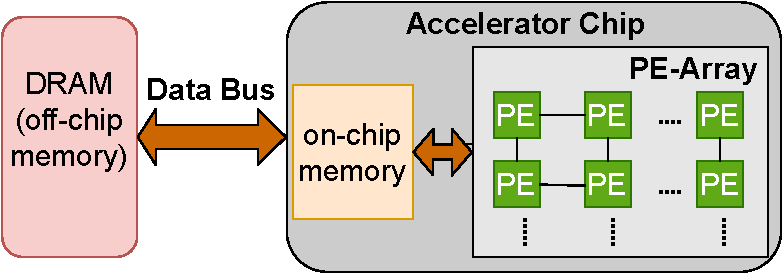
\includegraphics[width=0.5\textwidth]{typicalDNNAccelerator}
%	\caption{Typical DNN accelerator architecture}
%	\label{fig:typicalDNNAccelerator}
%\end{figure}
\begin{figure}[!htb]
	\centering
	\subfloat[]
	{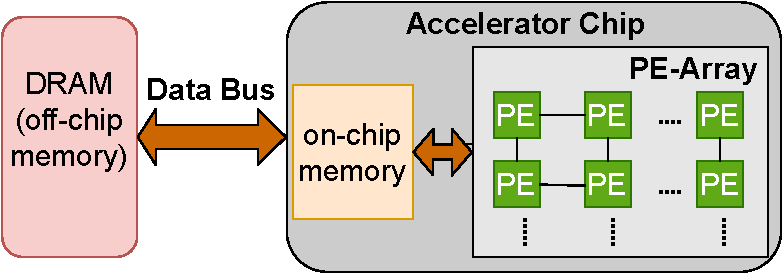
\includegraphics[width=0.4\textwidth]{typicalDNNAccelerator}
		\label{fig:typicalDNNAccelerator}}
	\hfil
	\subfloat[]
	{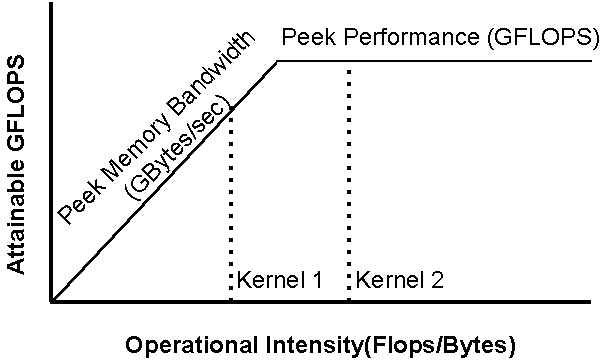
\includegraphics[width=0.35\linewidth]{roofline}
		\label{fig:roofline}}
	\caption{(a) Typical DNN accelerator architecture. (b) Roofline model}
	\label{fig:acceleratorAndRoofline}
	\vspace{-1.0em}	
\end{figure}

\figurename{~\ref{fig:typicalDNNAccelerator}} shows a typical DNN accelerator architecture, which consists of an off-chip memory and an accelerator chip. Accelerator chip mainly consists of an on-chip memory of few KBs and an array of Processing Elements (PEs). The accelerator system has multiple memory levels: off-chip memory, on-chip memory, and the registers inside the PE. Each memory level has different access latency and energy cost. The memory access energy from off-chip memory is upto two orders of magnitude higher than a PE computation operation~\cite{Chen2016EyerissAS}. It has been observed that more than 80\% of the overall energy consumption of these accelerators is due to off-chip memory accesses~\cite{chen2014diannao}. 

The PE-array (\figurename{~\ref{fig:typicalDNNAccelerator}}) has large number of processing elements, capable of performing several operations per cycle. However, throughput is often limited by off-chip memory bandwidth~\cite{williams2009roofline}. Fig.~\ref{fig:roofline} shows, two kernels (A and B) with different compute intensity (FLOPS/byte). Performance of kernels are limited by the memory bandwidth, which is typically the case for most of the DNN accelerators. Kernel B, applies data-reuse techniques to improve the computational intensity compared to kernel A and achieves better througput. Better data-reuse techniques are required to improve the performance on bandwidth-limited parallel architectures. 

Therefore, reducing the off-chip memory is the key to improve the throughput and energy efficiency of DNN accelerators. There are different types of neural networks. Recurrent Neural Networks (RNNs) and Convolutional Neural Networks (CNNs) are the most popular ones. Recurrent Neural Networks (RNNs) are widely used in sequential data processing applications such as speech recognition and natural language processing, while Convolutional Neural Networks (CNNs) are used in the area of computer vision e.g., image recognition. Each type of NN has its own challenges and require specific techniques to improve the performance. Towards this end we propose approaches to improve the performance of DNN accelerators for three popular NNs. Our main contributions in this thesis dessertations are
\begin{enumerate}
	\item We developed an offline-tool that computes the off-chip memory accesses of CNN layers, while considering the accelerator's architectural parameters. The offline-tool explores the large search space of tile dimensions and helpful in analysing the off-chip memory accesses for different data reuse schemes.
	\item We propose an approach that determines the optimal partitoning and scheduling scheme of the convolution (CL) and fully connected (FC) layers to mimimize the off-chip memory access and improve the energy-efficiency of CNN accelerators. We analytically express the off-chip memory accesses of CNNs  as a function of layer shapes, tiling parameters and the number of trips from the off-chip memory and express it as a constraint optimization problem. Using the above offline-tool we explore the design space to find the optimal solution. We implemented CL and FC layers on FPGA to demonstrate the efficacy of our approach compared to state of the art approaches.  
	\item We propose a novel data reuse approach to improve the throughput and energy efficiency of recurrent neural networks (RNNs). The proposed approach partitions the data and schedules the operations in a way that reduces the off-chip memory accesses of large matrices significantly. We implemented Long-Short Term Memory Network (LSTMs) accelerators for different approaches on FPGA to measure the design power and memory accesses and show the energy and througput improvements achieved by our approach.
	\item We analyse the effect of using different bit resolutions on the accuracy of a NN, as well as the benefits of using low bit width data resolution for self organizing maps (SOM) for designing a battery operated system where the area, power and performance are of critical importance. We implemented a SOM network on FPGA which can be configured for different bit resolution to compare the performace of different bit resolutions.
\end{enumerate}

\section{Related Work}
To address the computational and energy efficiency of DNNs, several ASIC~\cite{conti2018chipmunk,wang2017accelerating,azari2020elsa} and FPGA based accelerators~\cite{chang2015recurrent,ferreira2016fpga,lee2016fpga,guan2017fpga,han2017ese} are proposed. As off-chip memory accesses are the bottleneck in improving the throughtput and energy-efficiency of DNN accelerators, most of the recent works focused on reducing off-chip memory accesses. Some approaches~\cite{lee2016fpga, rybalkin2018finn, ferreira2016fpga} used on-chip memory to store all the weights. Sizes of weights in recent NN models can be several MB's, and using large on-chip memory is expensive. These approaches are not scalable and effective only for small NN models. 

There are two broad categories of work that aim to reduce the off-chip memory accesses of DNN accelerators as shown in Figure~\ref{fig:previousWorkClassification}. 
\begin{figure}[!htb]
	\centering
	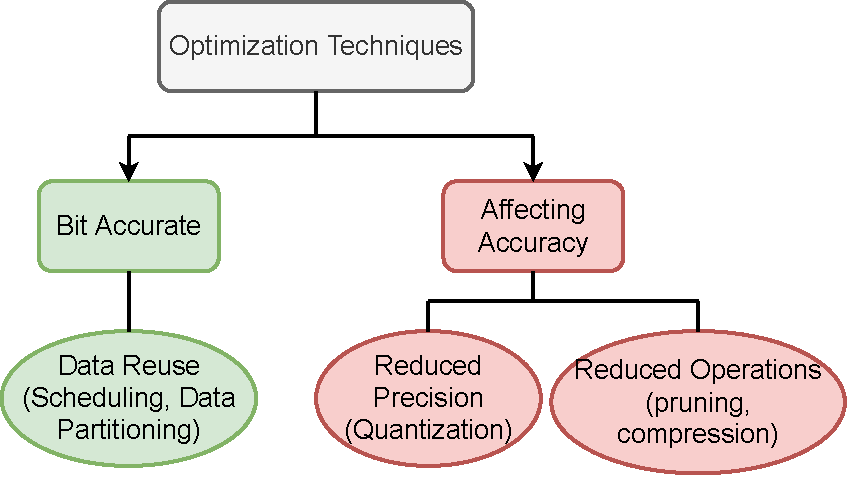
\includegraphics[width=0.5\textwidth]{previousWorkClassification}
	\caption{Broad Classification of previous works for improving the performance of DNN accelerators.}
	\label{fig:previousWorkClassification}
\end{figure}
One category of work exploits error-tolerence and redundancy in NNs using quantization and pruning techniques to compress the models' size. Approaches~\cite{ferreira2016fpga,wang2018c} used 18-bit, Chang et al.~\cite{chang2015recurrent} used 16-bit, Han et al.~\cite{han2017ese} used 12-bits precision for storing the inputs and weights, Lee et al.~\cite{lee2016fpga} used 8-bit inputs and 6-bits for weights to reduce the model size. 
Han et al.~\cite{han2017ese} used pruning to compress the model. However, pruning results in irregular network structure, and the sparse matrix require additional computational and storage resources and causes unbalanced load distribution. To overcome this Wang et al.~\cite{wang2018c} used block-circulant matrices representations to compress the LSTM/RNN model and to eliminate irregularities resulted from compression. Some approaches (\cite{park2019balancing,han2017ese,park2018maximizing}) used load balance aware pruning techniques to overcome the unbalanced load distribution problem. However, quantization and pruning approaches impacts the accuracy of the networks and may not be suitable where accuracy can not be compromised. 

The other category of works applies the data-reuse techniques to reduce the memory accesses without effecting the accuracy of the network. Zhang et al.~\cite{zhang2015optimizing} and Li et al.~\cite{Li2018SmartShuttleOO} used loop tiling and scheduling techniques to optimize the off-chip memory accesses of CNNs. Que et al.~\cite{que2019efficient} proposed a blocking-batching scheme to reuse the LSTM weights fetched from external memory. Park et al.~\cite{park2020time} proposed a time step interleaved weight reuse scheme (TSI-WR). 

We proposed data reuse approaches for state of the art CNNs and RNNs that are bit-accurate. These data-reuse approaches are orthogonal to the quantization techniques and can be integrated with different quantization techniques to reduce the memory accesses further. We have also analysed the impact of different bit-resolution on the accuracy of Self Organizing Maps (SOM) and to observe the improvements in the power, performance and area. 
\section{Optimizing the Performance of CNN Accelerators}
\subsection{Introduction}
Modern CNNs are very deep and have millions of parameters. To achieve high accuracy CNNs perform compute and memory intensive operations.  CNN accelerators exploits the parallelism to speed up the computations, however limited on-chip memory restricts the data reuse from on-chip memory. This results in large number of off-chip memory accesses, which degrades the performance and energy efficiency of CNN acclerators. 

CNNs have a sequence of mainly three types of layers: convolution layer (CL), pooling layer, and fully connected layer (FCL). There are several CLs, and a pooling layer usually follows each CL. The last few layers of the CNNs are FCLs. The computations of a CL and an FCL are illustrated in Figure~\ref{fig:CLOps} and~\ref{fig:FCLOps}, respectively. Each CL and FCL layer takes 3D input frames (\textit{ifm}) and applies filter weights (\textit{wts}) to compute output frames (\textit{ofm}).
\begin{figure}[!htb]
	\centering
	\subfloat[Convolution Layer]{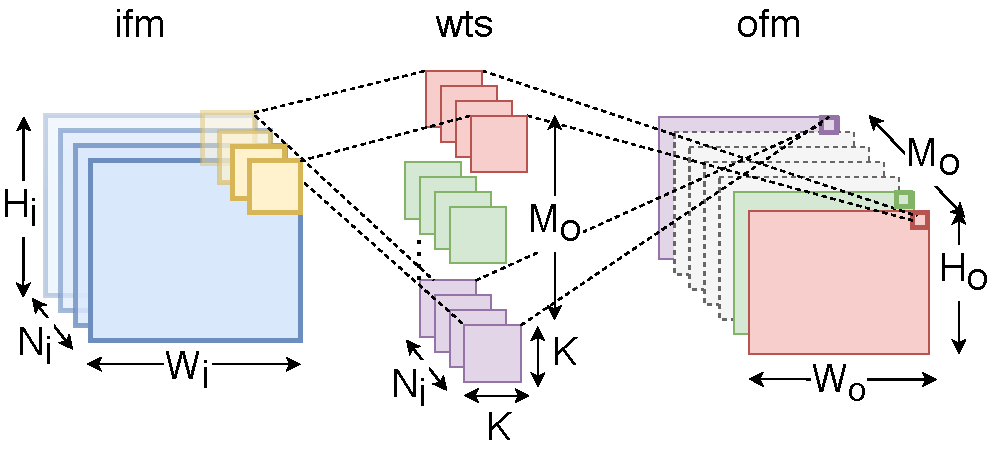
\includegraphics[width=0.49\textwidth]{CLOps.pdf}
		\label{fig:CLOps}}
	\hfil	
	\subfloat[Fully Connected Layer]{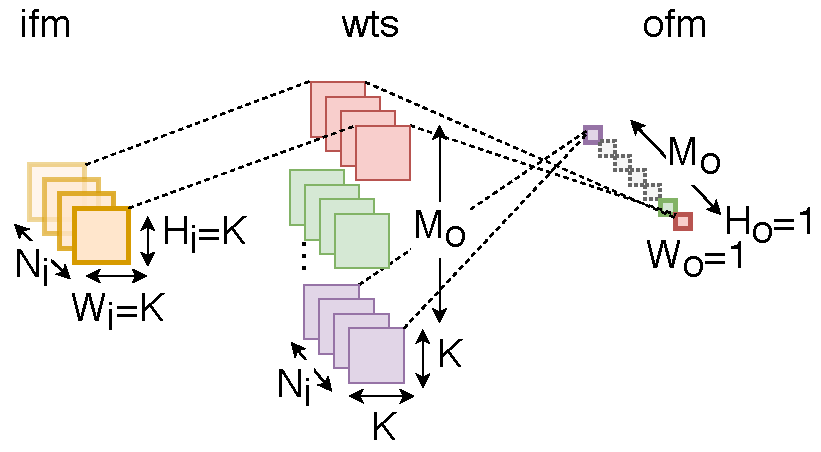
\includegraphics[width=0.42\textwidth]{FCLOps.pdf}
		\label{fig:FCLOps}}
	\hfil	
	\caption{Convolution and fully connected layers}
	\label{fig:CNNAcceleratorAndCLOps}
	\vspace{-1.0em}	
\end{figure}

CNN accelerators apply loop tiling to partition the layer data into small tiles that fits into on-chip memory. Loop tiling is a compiler  technique~\cite{aho2006compilers} that partitions the loop iteration space and large arrays into smaller tiles to increase the data locality and ensures that data fits into smaller memories. 
Fig.~\ref{fig:partitioningDataUsingTiling} shows a layer's data stored in off-chip memory and its tiles in the accelerator's on-chip buffer.
\begin{figure}[!htb]
	\centering
	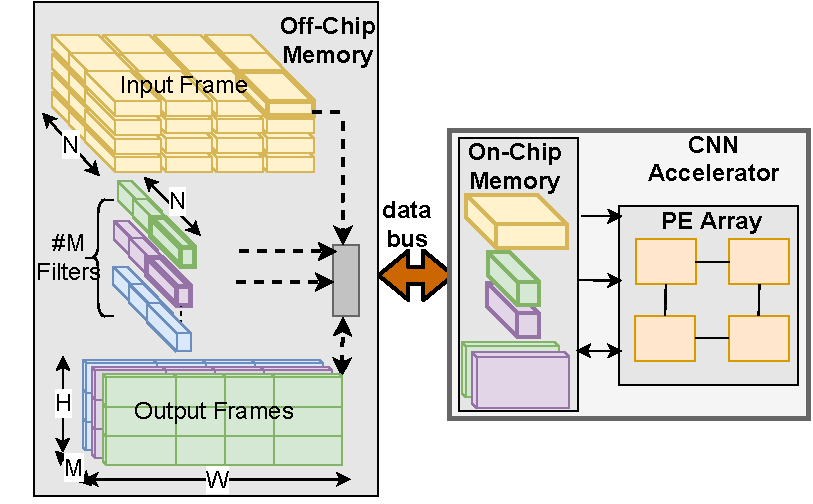
\includegraphics[width=0.5\textwidth]{images/AboutTheCNNTiles.pdf}
	\caption{CNN layer tiles in off-chip and on-chip memory}
	\label{fig:partitioningDataUsingTiling}
	\vspace{-1.0em}
\end{figure}
 The order of loops determines the scheduling of the tiles. The scheduling scheme, which minimizes the trips of the \textit{ifm} tiles between the accelerator and off-chip memory, is referred to as the input-reuse-oriented scheme (IRO). Similarly, the other two schemes, which minimize the trips of \textit{ofm} and \textit{wts} are referred to as output-reuse-oriented (ORO) and weight-reuse-oriented (WRO) scheme, respectively. The off-chip memory access depends on the data reuse scheme and the tile dimensions.  The tile dimensions significantly impacts the off-chip memory accesses~\cite{zhang2015optimizing, Li2018SmartShuttleOO}. 
   
CNN's layers have varying shapes. First few layers have large volume of \textit{ifm} and \text{ofm} and last few CLs and FCLs have large volume of \textit{wts}. The data reuse scheme optimal for one layer may be suboptimal for other layers due to varying layer shapes. In addition, memory accesses depend on the architectural parameters of the accelerator like bus width and data alignment. Our approach considers architectural parameters to compute the off-chip memory accesses and determines the optimal solution for each CL and FC layer.

\subsection{Related Work}
Zhang et al.~\cite{zhang2015optimizing} and Li et al.~\cite{Li2018SmartShuttleOO} used loop tiling to optimize the off-chip memory accesses. They expressed the off-chip memory access as a function of tile dimensions and layer shape. Zhang et al.~\cite{zhang2015optimizing} determined optimal tile dimensions by enumerating all the legal tile dimensions. To reduce the hardware design complexity, they determined a global optimal tile dimension and used a common data reuse scheme for all the layers. 
Li et al.~\cite{Li2018SmartShuttleOO} proposed a layer-wise adaptive data partitioning and scheduling scheme. However, their approach ignored the architectural parameters and address alignment, and assumed that all tiles of the same dimensions have the same off-chip memory accesses. With these assumptions, the tile dimensions determined by previous apporaches lead to a suboptimal solution.
\subsection{Off-Chip Memory Accesses of CNN Layers}
CNN accelerator access \textit{ifm}, \textit{ofm} and \textit{wts} of the layers from off-chip memory using loop tiling. Tiles are accessed multiple times from off-chip memory. The trips count depend on the data reuse scheme, layer shape, and tile dimensions. Trip counts of IRO, ORO, and WRO schemes can be expressed as the rows of the matrix \eqref{eq:TripCount}, where columns represent ifm, ofm, and weights.
\begin{align}\label{eq:TripCount}
	\mathbf{R}=
	\begin{bmatrix}
		\mathbf{r}_{iro} \\  \mathbf{r}_{oro} \\ \mathbf{r}_{wro} \\
	\end{bmatrix}= 
	\begin{bmatrix}
		1  & (2\ceil[\big]{\frac{N}{T_n}}-1) & \ceil[\big]{\frac{H}{T_r}} \ceil[\big]{\frac{W}{T_c}}\\[6pt]
		\ceil[\big]{\frac{M}{T_m}} & 1 & \ceil[\big]{\frac{H}{T_r}} \ceil[\big]{\frac{W}{T_c}}\\[6pt]
		\ceil[\big]{\frac{M}{T_m}} & (2\ceil[\big]{\frac{N}{T_n}}-1) & 1\\
	\end{bmatrix}
\end{align}
where $\langle T_{c_i},T_{r_i},T_{n_i}\rangle$, $\langle T_{c_o},T_{r_o},T_{m_o}\rangle$ and $\langle K,K,T_{n_i}\rangle$ are the tile dimensions, and $\langle W_i,H_i,N_i\rangle$, $\langle W_o,H_o,M_o\rangle$ and $\langle K,K,N_i\rangle$ are the data shape of \textit{ifm}, \textit{ofm} and \textit{wts}, respectively. The number of bytes accessed from off-chip memory ($\numBytesOffChip$) for a layer can be expressed as the following sum
\begin{equation}\label{eq:TotalOffChipAccess}
	\numBytesOffChip{}={}{r_{i}}{\cdot}\numBytesOffChip_{i}{+}{r_{o}}{\cdot}\numBytesOffChip_{o}{+}{r_{w}}{\cdot}\numBytesOffChip_{w}
\end{equation}
where $\numBytesOffChip_{i}$, $\numBytesOffChip_{o}$ and $\numBytesOffChip_{w}$ are the number of bytes accessed in one trip and $r_{i}$, $r_{o}$ and $r_{w}$ are the trips count of \textit{ifm, ofm} and \textit{wts} for the data reuse scheme, respectively. We compute the $\numBytesOffChip_{i}$, $\numBytesOffChip_{o}$ and $\numBytesOffChip_{w}$ for each layer considering the architectural parameters using equation~\ref{eq:accessfromUnalignedAddr}.

\subsubsection{Constraints}
The CNN accelerator stores the tiles of \textit{ifm}, \textit{ofm} and \textit{wts} in on-chip memory to perform the computations. Limited on-chip memory and the layer shape constraints the tile dimensions. Constraints are shown in~\eqref{eq:onChipConstraint} below
\begin{align}\label{eq:onChipConstraint}
	\begin{split}
		&(V_{i}{+}V_{o}{+}V_{w})\leq \BuffSize \\
		&0<T_{c_o}\leq W_o,~\ 0<T_{r_o}\leq H_o\\
		&0<T_{n_i}\leq N_i,~\ 0<T_{m_o}\leq M_o
	\end{split}
\end{align}
where $\BuffSize$ is the on-chip memory size and $V_{i}$, $V_{o}$ and $V_{w}$ are the \textit{ifm}, \textit{ofm} and \textit{wts} tile sizes computed as following 
\begin{align}\label{eq:tilesVol}
	\begin{split}
		V_{i}&=T_{c_i}{\cdot} T_{r_i}{\cdot} T_{n_i}{\cdot}\dataWidth\\
		V_{o}&=T_{c_o}{\cdot} T_{r_o}{\cdot} T_{m_o}{\cdot}\dataWidth\\
		V_{w}&=K^2{\cdot} T_{n_i}{\cdot} T_{m_o}{\cdot}\dataWidth
	\end{split}
\end{align}
where $\dataWidth$ is the data width in bytes.
Determining the optimal tile dimensions that minimizes $\numBytesOffChip$~\eqref{eq:TotalOffChipAccess}, is a constraint optimization problem. Equations~\eqref{eq:TotalOffChipAccess} and~\eqref{eq:onChipConstraint} are non linear and involve four variables $T_{c_o},T_{r_o},T_{n_i},T_{m_o}$. Thus it is not trivial to find the optimal solution.
\subsection{Impact of architectural parameters on memory access}\label{sec:OffChipAccessModel}
The CNN accelerators use a wide data bus to access off-chip memory to meet the high memory bandwidth requirement~\cite{Chen2016EyerissAS,chen2014diannao}. If the number of bytes accessed from an off-chip memory address is not a multiple of bus width or the address is not aligned to the word boundary, it results in unused bytes lanes of the data bus. Figure~\ref{fig:AXI_AccesseOn64BitDataBus} illustrates memory accesses on a 64-bit data bus.  Fig.~\ref{fig:AXI_AccesseOn64BitDataBus}a shows a read transaction of 8 bytes from an aligned address and uses the full bus width. However, if only 5 bytes are read from an aligned address, as shown in \figurename~\ref{fig:AXI_AccesseOn64BitDataBus}b, 8 bytes are still accessed. If 5 bytes are read from an unaligned address, it results in 16 bytes of data access, as shown in Fig.~\ref{fig:AXI_AccesseOn64BitDataBus}d. The unused byte lanes do not carry any useful data, but they contribute to overall energy consumption. The length of the data read should be chosen such that bus utilization is high, and off-chip memory accesses and energy consumption are minimized.
\begin{figure}[!htb]
	\centering
	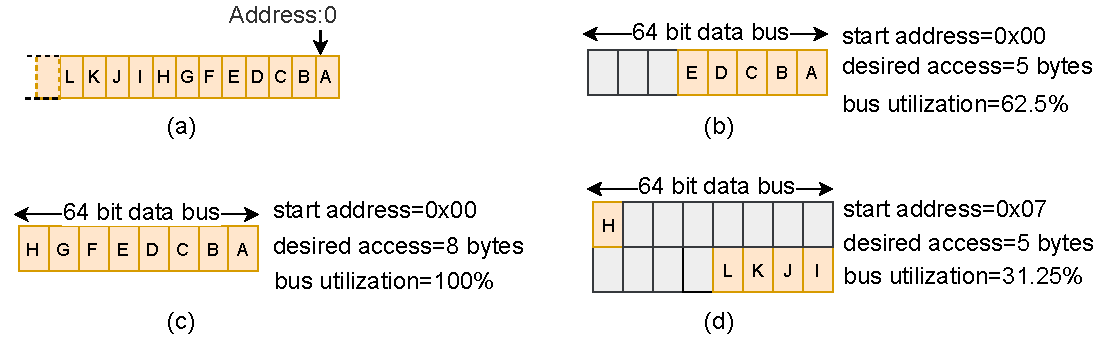
\includegraphics[width=0.7\textwidth]{./images/BurstTranscationOnAXI}
	\caption{Off-chip memory accesses on 64-bit wide data bus}
	\label{fig:AXI_AccesseOn64BitDataBus}
\end{figure}
The off-chip memory bus protocol supports burst based transactions where multiple data transfers of \emph{transfer size} happen from a starting address~\cite{AxiProtocolSpec}. Most transfers in a transaction are aligned to the \emph{transfer size}. However first transfer may be unaligned to the word boundary. 
The number of bytes accessed from off-chip memory ($\numBytesOffChip$) for accessing $\dataLength$ bytes from address $\addressSym$ on $\busWidth$ bytes of bus width can be expressed as
\begin{equation}\label{eq:accessfromUnalignedAddr}
	\begin{aligned}
		\numBytesOffChip(\addressSym,\dataLength,\busWidth)=(\ceil[\big]{\frac{\addressSym+\dataLength}{\busWidth}}-\floor[\big]{\frac{\addressSym}{\busWidth}})\cdot{\busWidth}
	\end{aligned}
\end{equation}
CNN accelerators access 3D data (ifm, ofm and weights) partitioned into tiles. We proposed a bus width aware approach (BWA) that factors in the architectural parameters to precisely compute the off-chip memory access of CNN layers.
\subsection{Offline-Tool For Design Space Exploration}
 Exploring design space of tile dimensions on hardware is time consuming and practically not possible. For a given CNN, the optimal tile dimensions and data reuse scheme need to be determined once. To determine the optimal tile dimensions, we have developed an offline tool that computes the off-chip memory access of CLs and FCLs of CNN which considering the architectural parameters as described in section~\ref{sec:OffChipAccessModel}
 \begin{figure}[!htb]
 	\centering
 	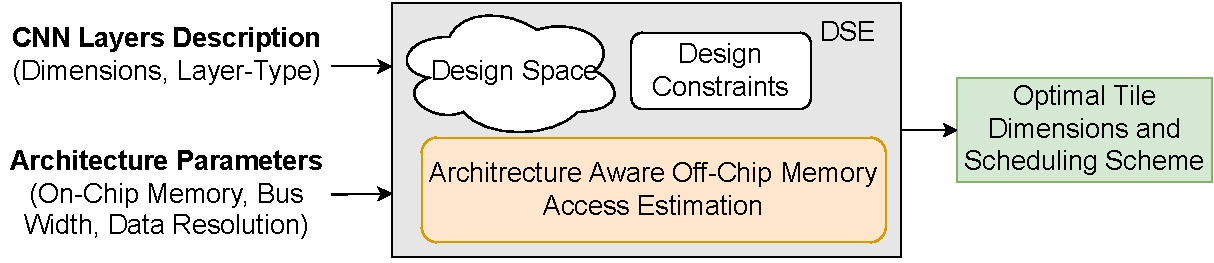
\includegraphics[width=0.7\textwidth]{offlineFrameworkForCNN}
 	\caption{Architecture Aware Offline-Tool for design space exploration}
 	\label{fig:offlineFrameworkForCNN}
 \end{figure}
 The tool takes layers description and architecture parameters as input and analyzes the off-chip memory accesses ($\numBytesOffChip$) for all feasible solutions that satisfy the constraints (\figurename~\ref{fig:offlineFrameworkForCNN}). The offline-tool can be configured for different on-chip buffer sizes, data reuse schemes, bus-width, data-resolution and determines each layer's optimal data reuse scheme and tile dimensions. The optimal solution determined by the offline-tool is then used in the CNN layers implementation on FPGA implementation to measure the energy and run-time. 
\subsection{Results}
We experimented with three popular CNN networks, AlexNet~\cite{krizhevsky2012imagenet}, VGG16~\cite{simonyan2014very}, and ResNet~\cite{he2016deep} having 8, 16, and 50 layers, respectively, with varying layer shapes and using filters of dimensions $1{\times}1$, $3{\times}3$, $5{\times}5$, $7{\times}7$, and $11{\times}11$. To compare the results with other approaches, we have used the on-chip buffer size of 108 KB, batch size of 3 for VGG16, and 4 for ResNet and AlexNet. 
\begin{figure}[!htb]
	\centering
	\subfloat[$\numBytesOffChip_{VGG16}$]
	{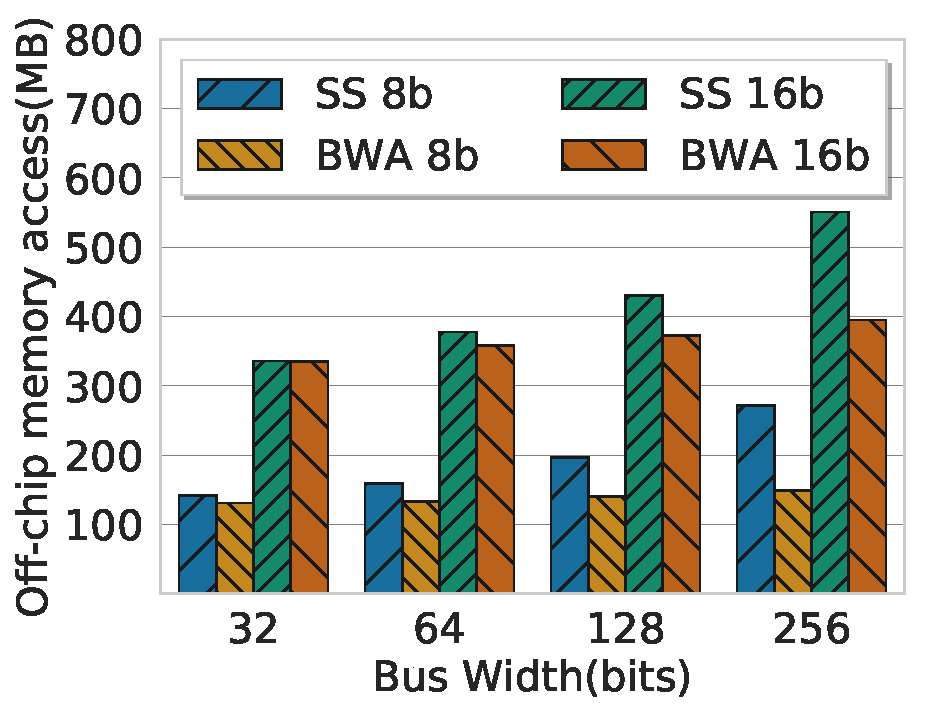
\includegraphics[width=0.32\textwidth]{VGG16_mem108_batch4_bw0_dW0_AD0.pdf}
		\label{fig:VGG16OffChipAccesses}}
	\hfil	
	\subfloat[$\numBytesOffChip_{AlexNet}$]
	{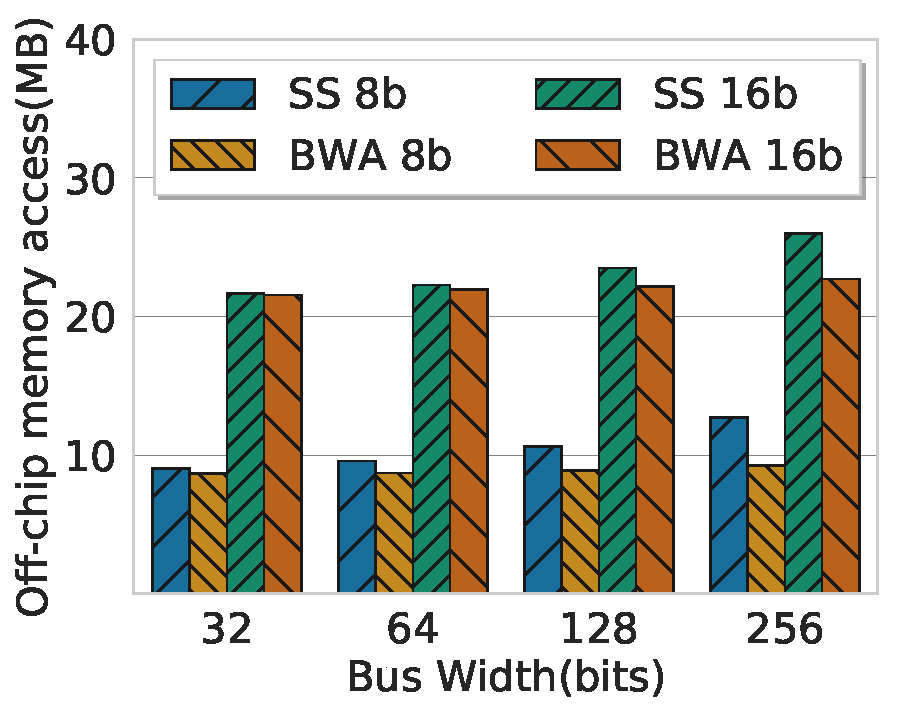
\includegraphics[width=.32\textwidth]{AlexN_mem108_batch4_bw0_dW0_AD0.pdf}
		\label{fig:AlexNetOffChipAccesses}}
	\hfil			
	\subfloat[$\numBytesOffChip_{ResNet}$]
	{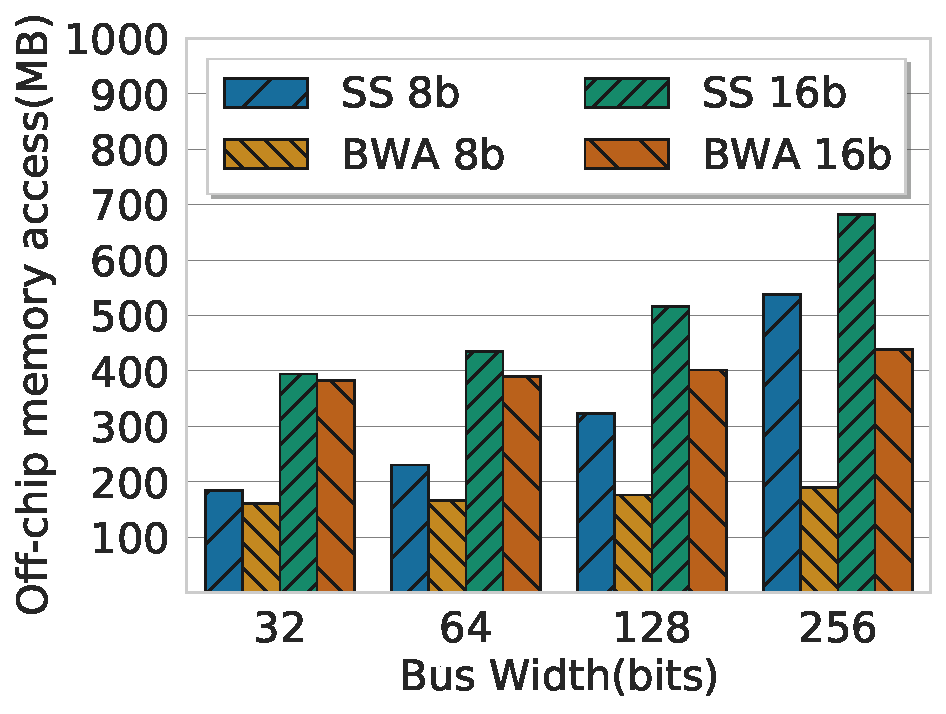
\includegraphics[width=.32\textwidth]{RESNet_mem108_batch4_bw0_dW0_AD0.pdf}
		\label{fig:ResNetOffChipAccesses}}
	\hfil	
	\caption{Off-chip memory access of convolution layers for 8 and 16 bits data width. BWA: Bus Width Aware, SS: SmartShuttle}
	\label{fig:AccessenOn64BitDataBus}
%	\vspace{-1.0em}
\end{figure}
Fig.~\ref{fig:AccessenOn64BitDataBus} shows the number of bytes accessed from off-chip memory ($\numBytesOffChip$) of CLs of the CNNs for different bus widths. $\numBytesOffChip$ is more for wider data buses because the overhead of unaligned access is more on a wider data bus. These unused bytes increase overall off-chip memory accesses. The proposed approach considers the bus width and addresses alignments to reduce the unaligned accesses. SS approach ignores architectural parameters and uses the same tile dimensions regardless of bus width, which results in increased off-chip memory accesses.
As shown in Fig.~\ref{fig:AccessenOn64BitDataBus}, our approach reduces $\numBytesOffChip$ compared to SS for the three CNNs. For ResNet:50 it reduces $\numBytesOffChip_{ResNet}$ by 13\%, 28\%, 46\%, and 65\% for 8 bits data width and by 10\%, 22\% and 36\% for 16 bits data width on 64, 128, and 256 bits wide data bus, respectively, compared to SS.
\begin{figure}[!htb]
	\centering
	\subfloat[]
	{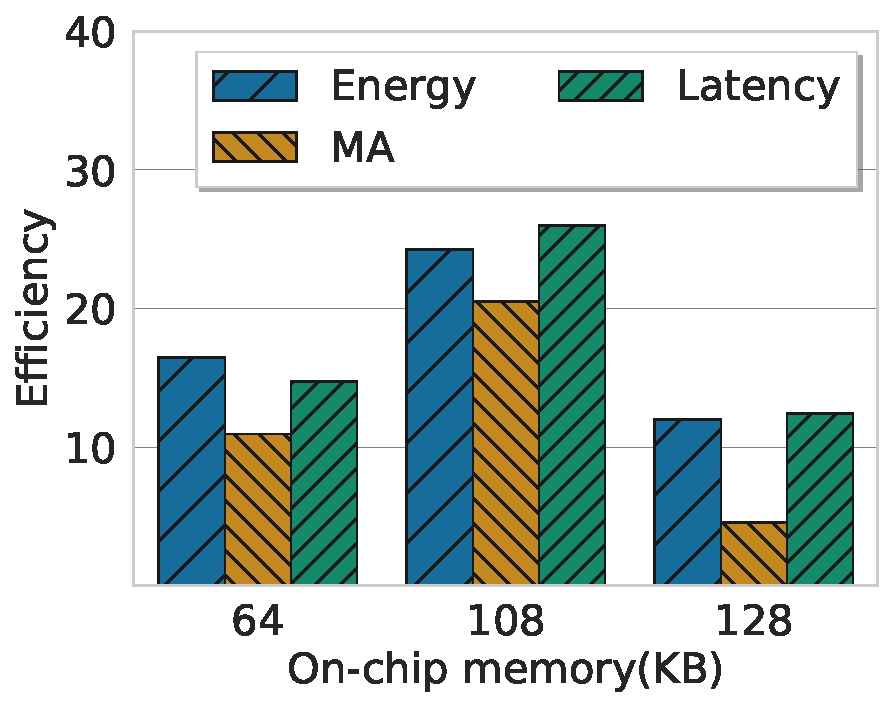
\includegraphics[width=0.32\textwidth]{energy_VGG16_DW8_BW64.pdf}
		\label{fig:VGG16EnergyEfficiency}}
	\hfil
	\subfloat[]
	{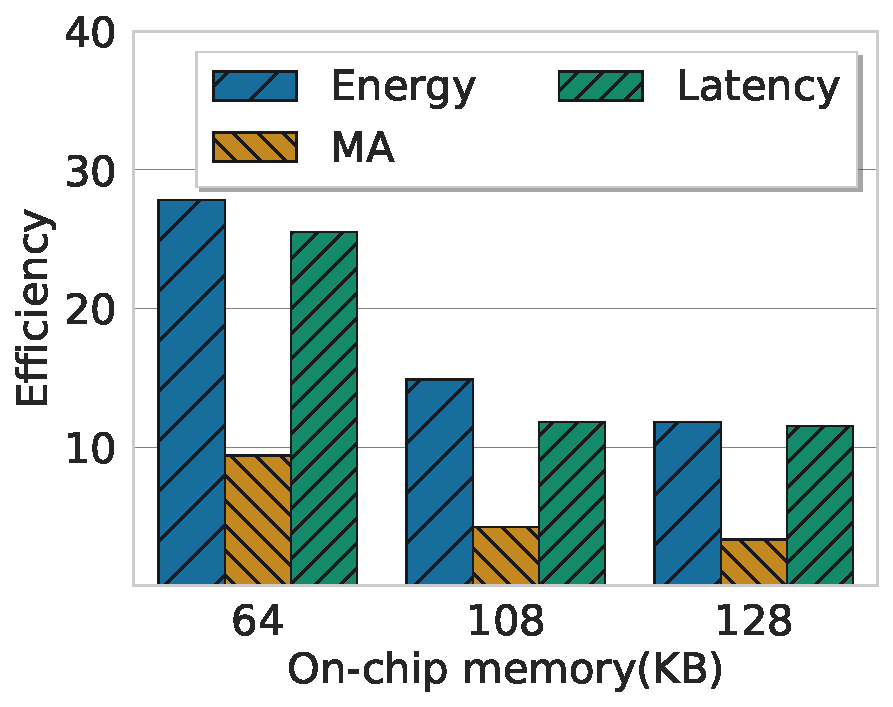
\includegraphics[width=0.32\textwidth]{energy_Alex_DW8_BW64.pdf}
		\label{fig:AlexEnergyEfficiency}}
	\hfil
	\caption{Energy and latency efficiency of BWA compared to SS. (a)VGG16, (b)AlexNet}
	\label{fig:EffectOnLatency}
	%	\vspace{-1.0em}
\end{figure}

\figurename{~\ref{fig:VGG16EnergyEfficiency}} and \figurename{~\ref{fig:AlexEnergyEfficiency}} show the energy, off-chip memory accesses, and latency efficiency achieved using the BWA compared to the SS approach for VGG16 and AlexNet, respectively, for 8 bits data width and 64 bits bus width. We observed that the changes in energy and latency are proportional to the changes in memory access. This observation confirms that off-chip memory access dominates the energy consumption of the CNN accelerators.
\section{Optimizing the Performance of RNN/LSTM Accelerators}
\subsection{Introduction}
Many applications involve sequential data processing and time-series predictions, e.g., natural language processing, speech recognition, video activity recognition. Processing sequential data requires remembering the contextual information from previous data. Recurrent neural networks (RNNs) are specialized in handling such problems by maintaining an internal state based on previously seen data. LSTMs \cite{hochreiter1997long} are variants of RNNs designed to handle long-range dependencies by storing useful information about previous inputs for a long duration. 

Typically the computations of LSTM cell is described by the following equations
\begin{align}\label{eq:lstmEqs}
	\begin{split}
		&i{=}{\sigma}(W^i{\cdot}x_t{+}R^i{\cdot}h_{t-1}{+}b^i)\\
		&f{=}{\sigma}(W^f{\cdot}x_t{+}R^f{\cdot}h_{t-1}{+}b^f)\\
		&g{=}{\tanh}(W^g{\cdot}x_t{+}R^g{\cdot}h_{t-1}{+}b^g)\\
		&o{=}{\sigma}(W^o{\cdot}x_t{+}R^o{\cdot}h_{t-1}{+}b^o)\\
		&c_{t}{=}f{\odot}c_{t-1}{+}i{\odot}g\\
		&h_{t}{=}o{\odot}{\tanh}(c_t)
	\end{split}	
\end{align}
where $x_t$ is the input, $h_t$ is the hidden state, and $c_t$ is the cell state at time $t$. $i,f,g,o$ are the computed gate values at time t. $\odot$ denotes the element-wise multiplications. $W^j$ and $R^j$ are the input and hidden state weight matrices, and $b^j$ is the bias vector, learned during the training process, where $j\in\{i,f,g,o\}$. The dimension of $h_t$ is referred to as the number of hidden states of the LSTM ($N$). 
At every time step, $x_t$ is taken as input, and $c_t$ and $h_t$ are computed using Equation~\eqref{eq:lstmEqs}. The dependency of $h_t$ on $h_{t-1}$ and $c_{t-1}$ prevents the parallel processing of multiple time steps and limits the data reuse. 

LSTM computations involve multiple matrix-vector multiplications, and these matrix-vector multiplications are performed for large number of time-steps. The size of matrices can be significant in several MB's and often exceed the size of the accelerator's on-chip memory. These matrices are partitioned into blocks and accessed from off-chip memory repeatedly by the accelerator, which results in a large volume of off-chip memory accesses and energy consumption.
\begin{figure}[!htb]
	\centering
	\subfloat[Conventional approaches: $R$ matrix is accessed at each time step.]
	{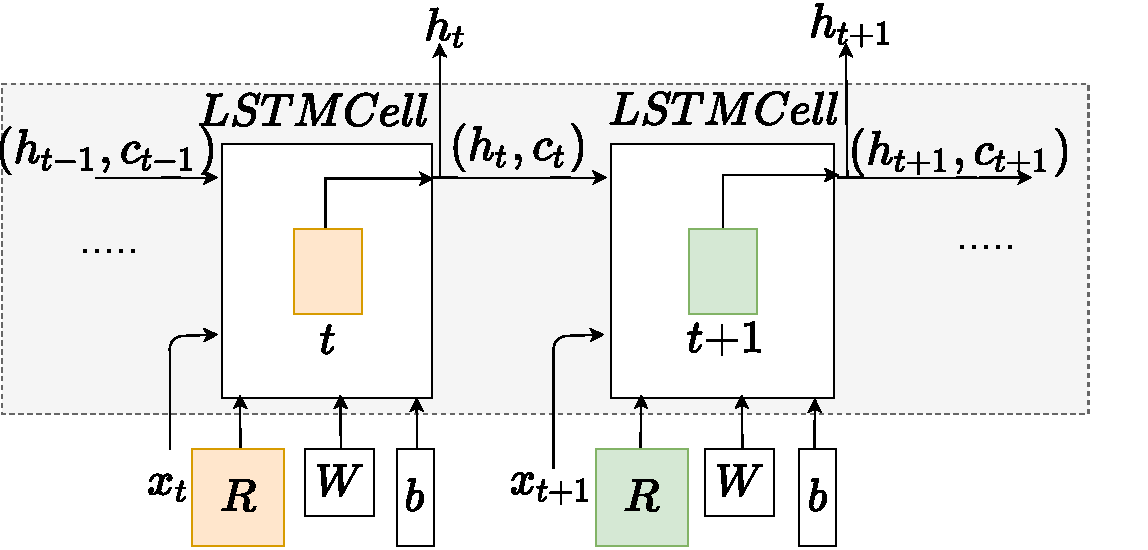
\includegraphics[width=0.4\textwidth]{introA.pdf}
		\label{fig:introA}}
	\hfil
	\subfloat[Proposed approach: $R$ matrix accesses are reduced by half. ]
	{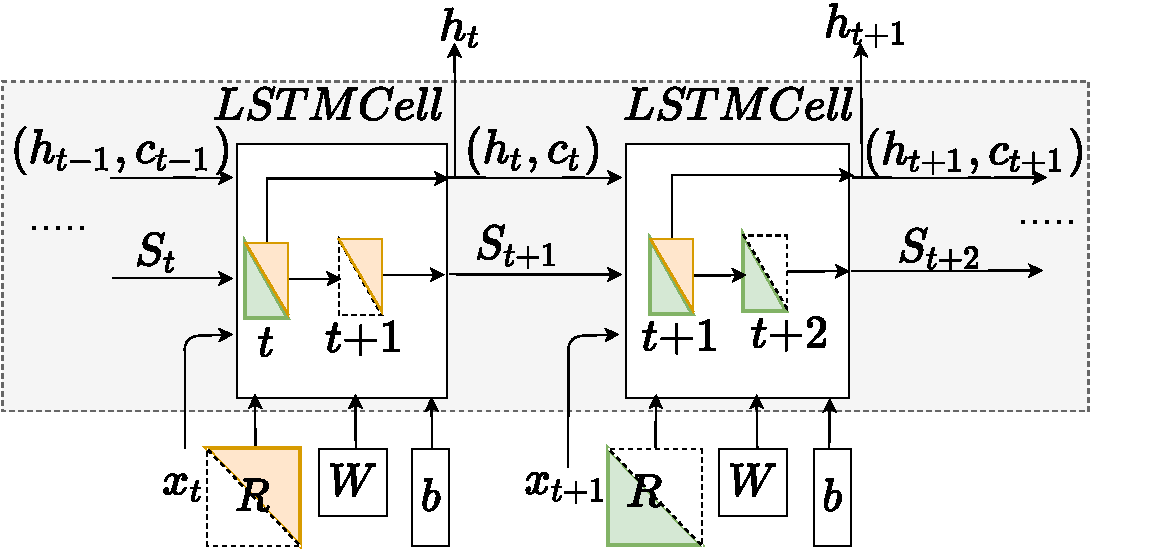
\includegraphics[width=.4\textwidth]{introB.pdf}
		\label{fig:introB}}
	\hfil	
	\caption{LSTM cell computations for consecutive time-steps showing the weight accesses.}
	\label{fig:introToApproach}
	\vspace{-1.0em}	
\end{figure}
Figure{~\ref{fig:introToApproach}} shows the LSTM cell computations for two consecutive time steps using  conventional and the proposed approach. To compute the hidden state vector $h_t$, conventional approaches accesses $R$ matrix at each time step $t$, as shown in Fig.{~\ref{fig:introA}}. Accessing the weights at each time step results in large volume of off-chip memory accesses. We propose an approach that reduces off-chip memory accesses by splitting the computation in two, as shown in~\figurename{~\ref{fig:introB}}. At each time step, while the computations of a hidden state vector of one time step $h_t$ completes, partial computation of next time step ($S_{t+1}$) is also performed by reusing the weights, which reduces the $R$ matrix accesses by approximately half. The data reuse in our approach is independent of on-chip buffer sizes which makes it suitable for small on-chip memory accelerators.
\subsection{Related Work}
The matrix-vector multiplication $W^j\cdot x$ in Equation~\eqref{eq:lstmEqs}, where $j\in \{i,f,g,o\}$, is independent of previous state computation. Que et al.~\cite{que2019efficient} proposed a blocking-batching scheme which reuses the weights of $W^j$ matrix by processing group of input vectors as a batch. The input vectors in the same batch share the same weight matrices ($W^j$). However, it is difficult to collect required number of input vectors. As the LSTM cell states ($h_t$ and $c_t$) computations depend on previous time-step cell states, benefit of their batching schemes is limited to $W^j\cdot x$. Reusing weights of $R$ across different time-steps has not been successful because of the dependency on previous time-step states.

Park et al.(~\cite{park2020time}) proposed a time step interleaved weight reuse scheme (TSI-WR) which reuses the weights of $R$ matrix between two adjacent time steps by performing computations in a time-interleaved manner. Their approach logically partitions the $R$ matrix into blocks. A block is accessed from off-chip memory to compute the hidden state vector $h_t$, a fraction of it is reused to compute the partial sum of next time step state $h_{t+1}$. However, their approach do not fully exploit the data reuse, and several weights are accessed repeatedly from the off-chip memory. In addition, the data reuse in TSI-WR approach depends on the on-chip storage size which limits the benefits of their approach to accelerators with larger on-chip memory.
\subsection{Proposed data reuse approach}
The computation of the $h_t$ can be expressed as shown below
\begin{align}\label{eq:h_{t}}
	h_{t}[k] &= F( S_{t}[k]+q_{t}[k])
\end{align}
where $F$ is a non-linear function. $q_{t}$ is computed as $W{\cdot}x_t{+}b$ and its computations are independent of previous step cell states. $S_{t}[k]$ is the sum of $N$ product terms as shown below,
\begin{align}
	S_{t}[k] = \sum_{n=0}^{N-1}R[k][n]\cdot h_{t-1}[n]
\end{align}
$S_{t}[k]$ can be computed as a sum of the following two partial sums $S_{t}^{L}[k]$ and $S_{t}^{U}[k]$
\begin{align}      
	S_{t}^{L}[k] &= \sum_{n=0}^{k}R[k][n]\cdot h_{t-1}[n] \label{eq:S_L_{t}}\\
	S_{t}^{U}[k] &= \sum_{n=k+1}^{N-1}R[k][n]\cdot h_{t-1}[n] \label{eq:S_U_{t}}
\end{align}
Equation~\eqref{eq:S_L_{t}} uses the lower-diagonal and diagonal elements of $R$ ($R^L$), and~\eqref{eq:S_U_{t}} uses the upper diagonal elements of $R$ ($R^U$). 
\begin{figure}[!htb]
	\centerline{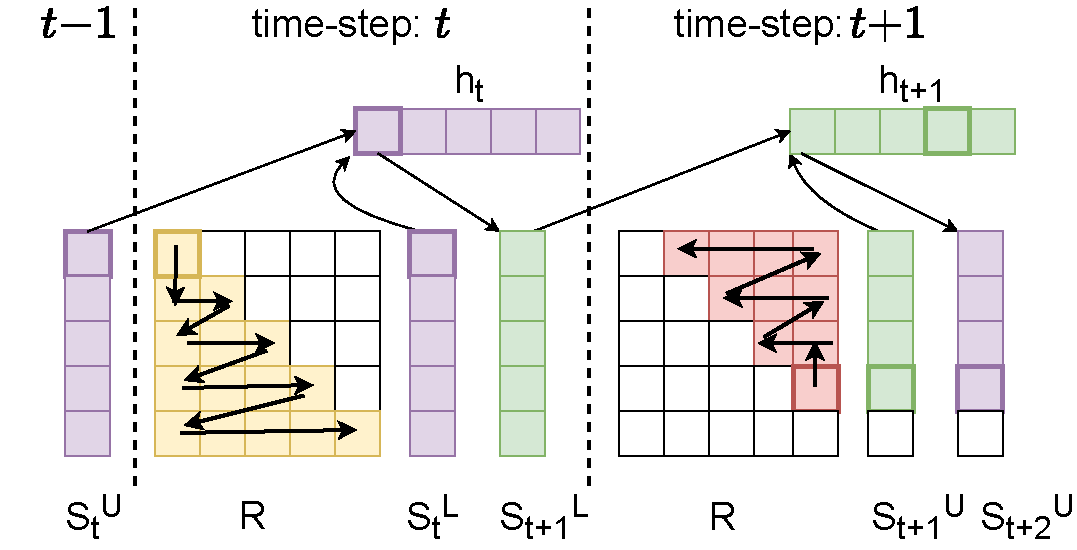
\includegraphics[width=0.5\textwidth]{TwoTimeSteps.pdf}}
	\caption{Splitting the hidden state vector computations into partial sums}
	\label{fig:TwoTimeStepsComputation}
	\vspace{-1.0em}	
\end{figure}
As shown in \figurename{~\ref{fig:TwoTimeStepsComputation}}, $R^L$ and $R^U$ are accessed in consecutive time steps and reused in the partial sum computations of two steps. 
%At time step $t$, $S_t^U$ and $h_{t-1}$ are the inputs from the previous time step, and $R^L$ is reused to compute the partial sums $S_{t}^{L}$ and $S_{t+1}^L$. Input $S_{t}^{U}$ is added to $S_{t}^{L}$ to compute $h_{t}$, and $S_{t+1}^L$ is passed to $(t{+}1)^{th}$ step computations.
%In the same way, at time step $t{+}1$, $R^U$ is reused to compute $S_{t+1}^{U}$ and $S_{t+2}^{U}$.
Elements of $R^L$ are accessed from top to bottom, left to right, while elements of $R^U$ are accessed in the reverse order to satisfy the dependencies. As shown in~\figurename{~\ref{fig:TwoTimeStepsComputation}}, the proposed approach accesses the weight matrix $R$ once, to compute the output of two consecutive time steps $h_{t}$ and $h_{t+1}$. 
\subsection{Results}
We have compared our approach with conventional approaches and state of the art TSI-WR approach~\cite{park2020time}. We have used the same on-chip buffer size to store the weight matrices to perform a fair comparison. The proposed approach requires additional $4N$ elements storage for the partial sum vectors. We have experimented with LSTM models used in speech recognition (for TIMIT~\cite{garofolo1993timit}) and character level Language Modelling (LM)~\cite{sundermeyer2015feedforward}.
\begin{figure}[htb!]
	\centering
	\subfloat[]
	{
		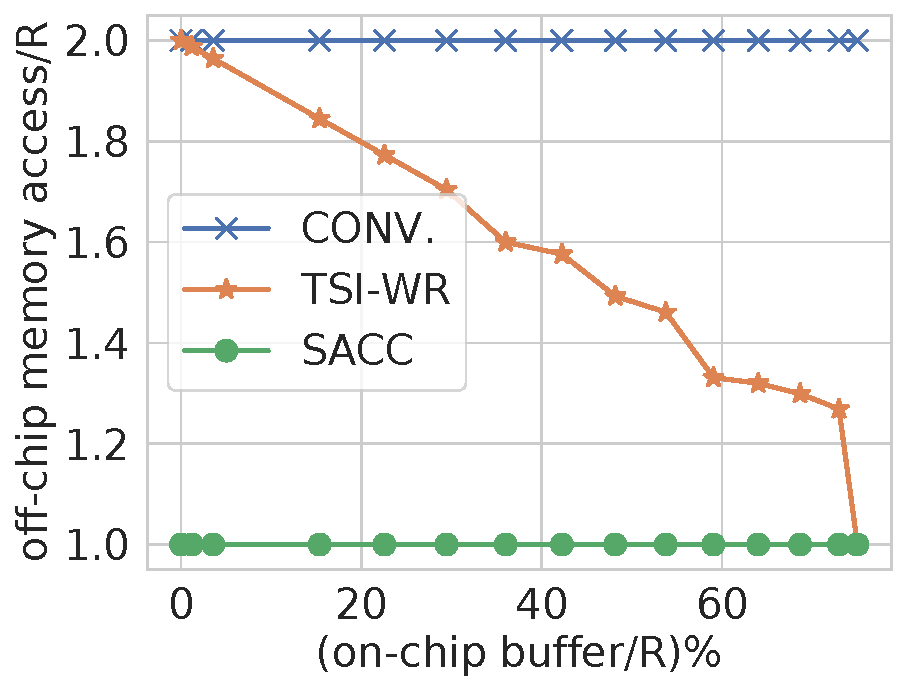
\includegraphics[width=0.32\textwidth]{tsiwrComparisonModified.pdf}
		\label{fig:compareWithTSIWR}
	}	
	\subfloat[]
	{
		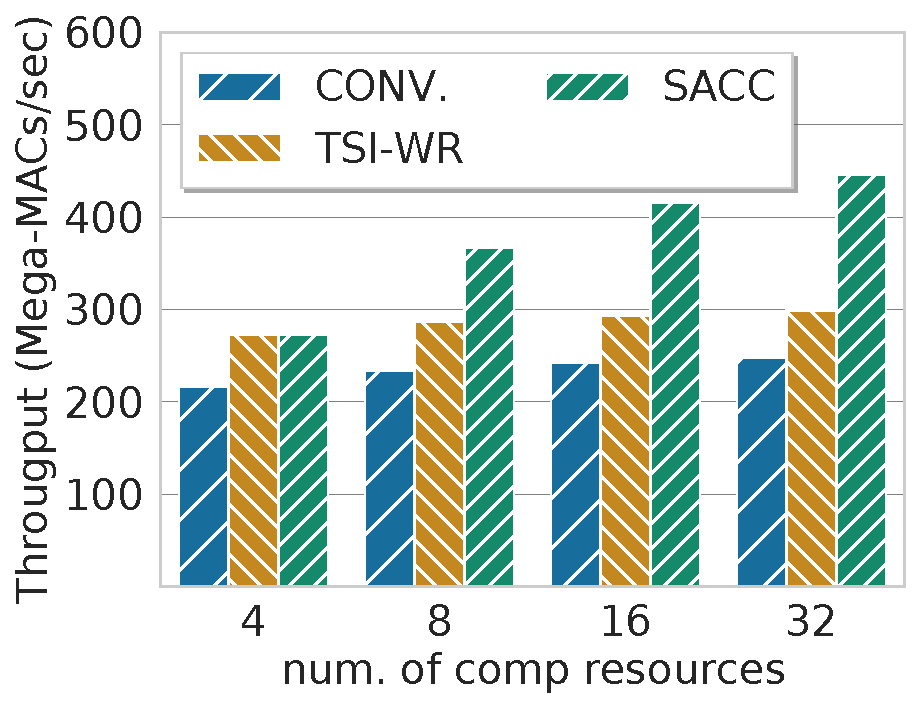
\includegraphics[width=0.32\textwidth]{througput_N256.pdf}
		\label{fig:throughPutVsPF_128}
	}
%	\subfloat[]
%	{
%	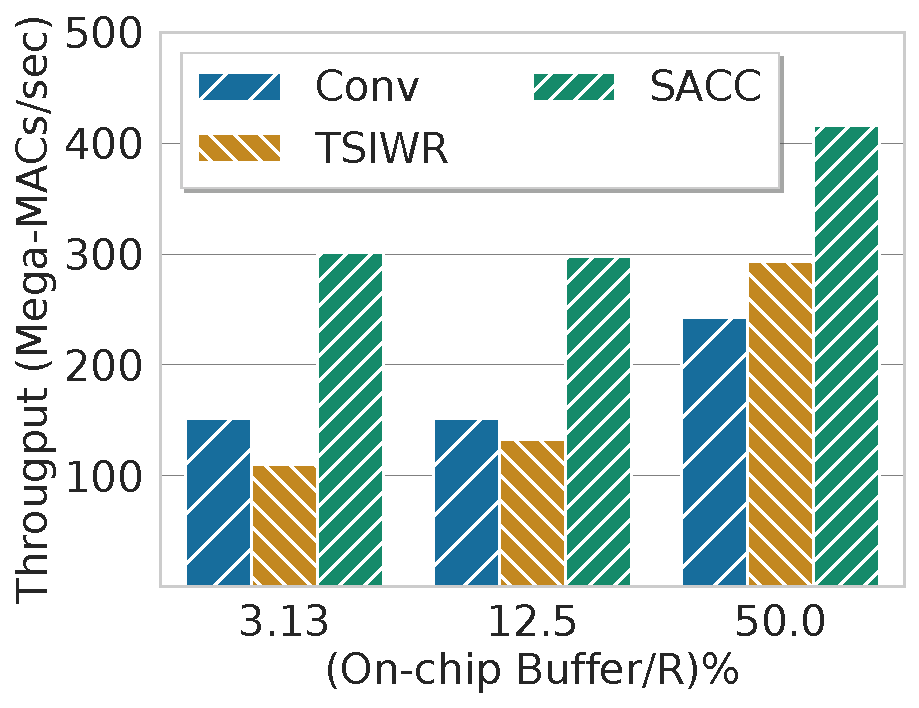
\includegraphics[width=0.23\textwidth]{througputVsMem_128KB.pdf}
%	\label{fig:throughPutVsMem_128}
%	}
	\subfloat[]
	{
	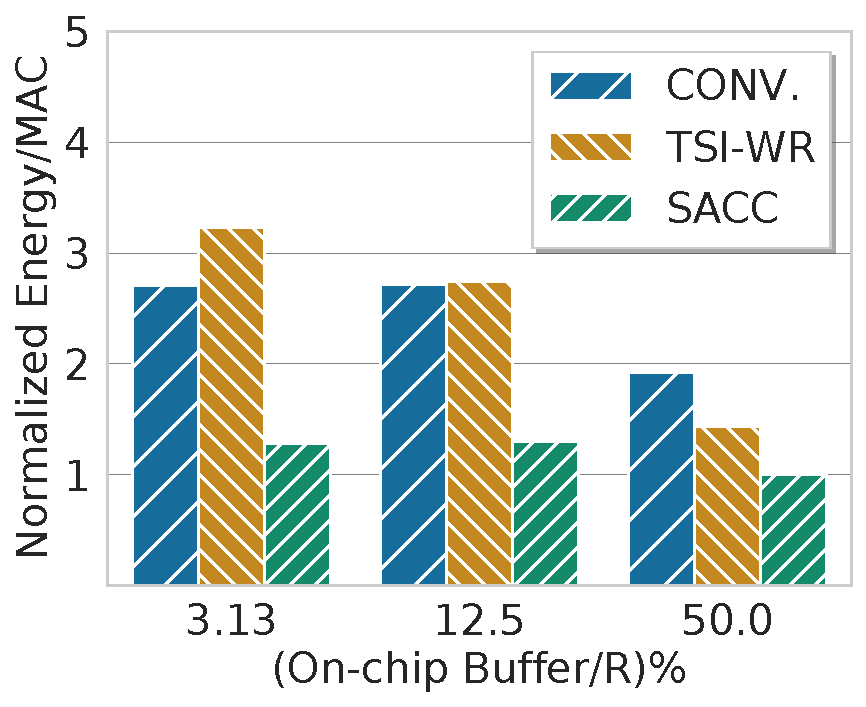
\includegraphics[width=0.32\textwidth]{energyVsMem_128KB.pdf}
	\label{fig:energy_128}
	}
	\caption{ (a) Off-chip memory accesses for matrix-vector multiplication (MxV) of two consecutive time-steps with different on-chip buffer/R ratio, (b) Throughput variation of MxV for different compute resources for (on-chip buffer/matrix size){=}0.5, (c) Energy improvement for different on-chip buffer size/R ratio.}
	\label{fig:throughputVsPF}
	\vspace{-1.0em}	
\end{figure}
\subsubsection{Memory Accesses}
\figurename{~\ref{fig:compareWithTSIWR}} compares the off-chip memory accesses of the proposed (SACC), conventional and the TSI-WR approaches. Conventional approaches access the full matrix $2{\times}R$ at each time step. For the TSI-WR approach data reuse depends on on-chip buffer sizes. For larger on-chip buffer sizes the data reuse is more. When the on-chip buffer size is 70\%, TSI-WR approach reduced 50\% off-chip memory accesses compared to conventional approach. However, for smaller on-chip buffer sizes the reduction is less. The proposed approach reduces memory access of $R$ matrix by 50\%, irrespective of the on-chip buffer size.
\subsubsection{Througput Improvement}
Off-chip memory bandwidth typically limits the performance of LSTM/RNN accelerators. Increasing the number of computing resources does not improve the performance for the conventional approaches, as shown in \figurename{~\ref{fig:throughPutVsPF_128}}. TSI-WR approach improves the throughput with increasing the number of compute resources. However, throughput improvement in the TSI-WR approach is observed only for the large on-chip buffer to matrix size ratio. \figurename{~\ref{fig:throughPutVsPF_128}} shows the results for on-chip buffer to matrix size ratio of 50\%. The proposed approach, always reuses the data for two time step computations, which results in throughput improvement with increasing the number of parallel resources.
\subsubsection{Energy Efficiency}
\figurename{~\ref{fig:energy_128}} shows the normalized energy efficiency per MAC operation for different on-chip buffer to R matrix size ratios for 128~KB on-chip buffer sizes. Increasing the on-chip buffer size to matrix size ratio improves the energy-efficiency for all the three approaches. For smaller on-chip buffer to R matrix size ratios conventional approach performs better than TSI-WR due to their simpler control logic. For large on-chip buffer sizes, TSI-WR outperforms the conventional approaches. Out of all the three approaches, the proposed approach performs better than the other two approaches for all the on-chip buffer size ratios. For 50\% on-chip buffer to matrix size ratio, the SACC approach reduces 48\% and 30\% energy compared to conventional and TSI-WR approach, respectively.

%\section{Analysing the impact of Low Bit-Width on the performance of SOMs}
\section{Performance Improvement of SOM by using Low Bit-Width Resolution}
\subsection{Introduction}
One of the popular low-power stategy is performing computations at reduced bit-widths by trading off accuracy. The benefits of using reduced bit-width results in improved energy performance metrics. This is because there is a reduction of the energy cost for data transfers, which usually dominates the total energy consumption for such systems.

%In this work, we explore the impact of different bit resolutions on the accuracy, as well as the benefits that this low resolution can provide for a hardware architecture. We have done hardware implementation of SOM on FPGA, mapped on Xilinx Virtex7 485t chip, handcrafted for different bit width implementations to analyze the area vs energy trade off.
We explored the design space of a self-organizing map (SOM) to analyse the impact of different bit resolutions on the accuracy, as well as its benefits. SOM uses a type of unsupervised learning called competitive ANN learning model. We have implemented SOM on FPGA and to lower the energy consumption, we exploit the robustness of SOM by successively lowering the resolution to gain in efficiency and lower the implementation cost. We do an in depth analysis of the reduction in resolution vs. loss in accuracy. The objective of this method is to design a bacterial recognition system for battery operated clinical use where the area, power and performance are of critical importance. We demonstrate that with 39\% loss in accuracy in 12 bits and 1\% in 16 bit representation can yield significant savings in energy and area.

%Prior work in \cite{Yang2018RiBoSOM} has introduced Self-organizing maps (SOM) for rapid genome identification. SOM uses a type of unsupervised learning called competitive ANN learning model. The model reduces the data dimensions and it clusters similar data together \cite{Kohonen2013}. A trained SOM network does not require to go through the whole DNA sequence to recognize the pathogen, but only requires a small part of its DNA. SOM can be highly parallelized and such parallel implementation have been proposed for synchoros VLSI design, custom FPGA and GPUs \cite{Yang2018RiBoSOM, Porrmann2006, McConnell2012}. Another important aspect of SOM and other ANN is their robustness. ANNs have been proven to work with low bit resolution without sacrificing much of their accuracy \cite{8056820}. In this work, we explore the limits of the SOM using different bit resolutions and the effect that it has on the accuracy of the SOM, as well as the benefits that this low resolution can provide for a hardware architecture. 

\subsection{Related Work}
 An emerging design paradigm that is able to achieve better energy efficiency by trading off the quality (e.g., accuracy) and effort (e.g., energy) of computation is approximate computing~\cite{Zhang2014}. Many modern applications, such as machine learning and signal processing, are able to produce results with acceptable quality despite most of the calculations being computed imprecisely~\cite{Ye2013}. The tolerance of imprecise computation in approximate computing  to acquire substantial performance gains and is the basis for a wide range of architectural innovations~\cite{Esmaeilzadeh2012}.


%Earlier work in approximate computing was focused on the design of basic elements, such as approximate adders and logic~\cite{Gupta2012}.  Although, these techniques  adequately demonstrated the benefit of approximate computing,  the fixed functionality and low-level design limits further performance improvement. Additionally, many of these techniques use complementary metal-oxide-semiconductor (CMOS) technology. Innovations in   device technology  provide a great opportunity for radically different forms of architecture design~\cite{Venkataramani2012}.

%One of the  popular low-power strategy implemented in custom designs consists in performing computations at reduced bit-widths. In some cases, this results in  trading off accuracy for smaller power consumption. The  benefits of doing this results in improved energy performance metrics in both the data path and in the memory path. This is because  there is a  reduction of the energy cost for data transfers, which usually dominates the total energy consumption for such systems. Machine learning tasks do have intrinsic error resilience  and hence it is expected that bit-width reduction will  work well 

Previous works has demonstrated that high-precision computations are often unnecessary in presence of statistical algorithms~\cite{Moons2017,Zhang2015}. Znag et.al. report a less than 5\% of quality loss  obtained by simulation of the real hardware implemented in a 45nm CMOS technology. Gupta et. al. also present similar results where they train deep networks with 16 bits fixed-point number representations and stochastic rounding~\cite{Gupta2015}. Talathi et. al. show that  the best performance with reduced precision  can be  achieved with 8 bits weights and 16 bits activation, which, if reduced to 8 bits, results in  a 2\% drop in accuracy. Hashemi et. al. look at a broad range of numerical representations applied to ANNs in both inputs and network parameters and analyze the trade-off between accuracy and hardware implementation metrics and conclude that a wide range of approximation parameters are feasible with negligible degradation in performance~\cite{Hashemi2017}.

\subsection{Low bit-width FPGA Design of SOM}
We have implemented SOM on FPGA, mapped on a Xilinx Virtex7 485t chip, for identification of bacterial genomes. A custom semi systolic array was hand crafted, for different bit width implementations, to analyze the area versus energy trade off.

Figure \ref{fig:algo} shows a high level schematic of the FPGA implementation of BioSOM and illustrates the key components in the design. The input is a $n$-bit vector. Each pair of bits in the input represents one of nucleotide A,C,G or T. Thus a 16-bit word contains 8 symbols.  The Neural Network weights are stored in BRAMs. Each neuron has 8 weights and each weight is stored as a fixed-point number. Bit width analysis is performed by varying the number of bits (8, 12, 16, 24 and 32) used to represent the weights.

\begin{figure}[!htb]
	\centering
	\subfloat[]
	{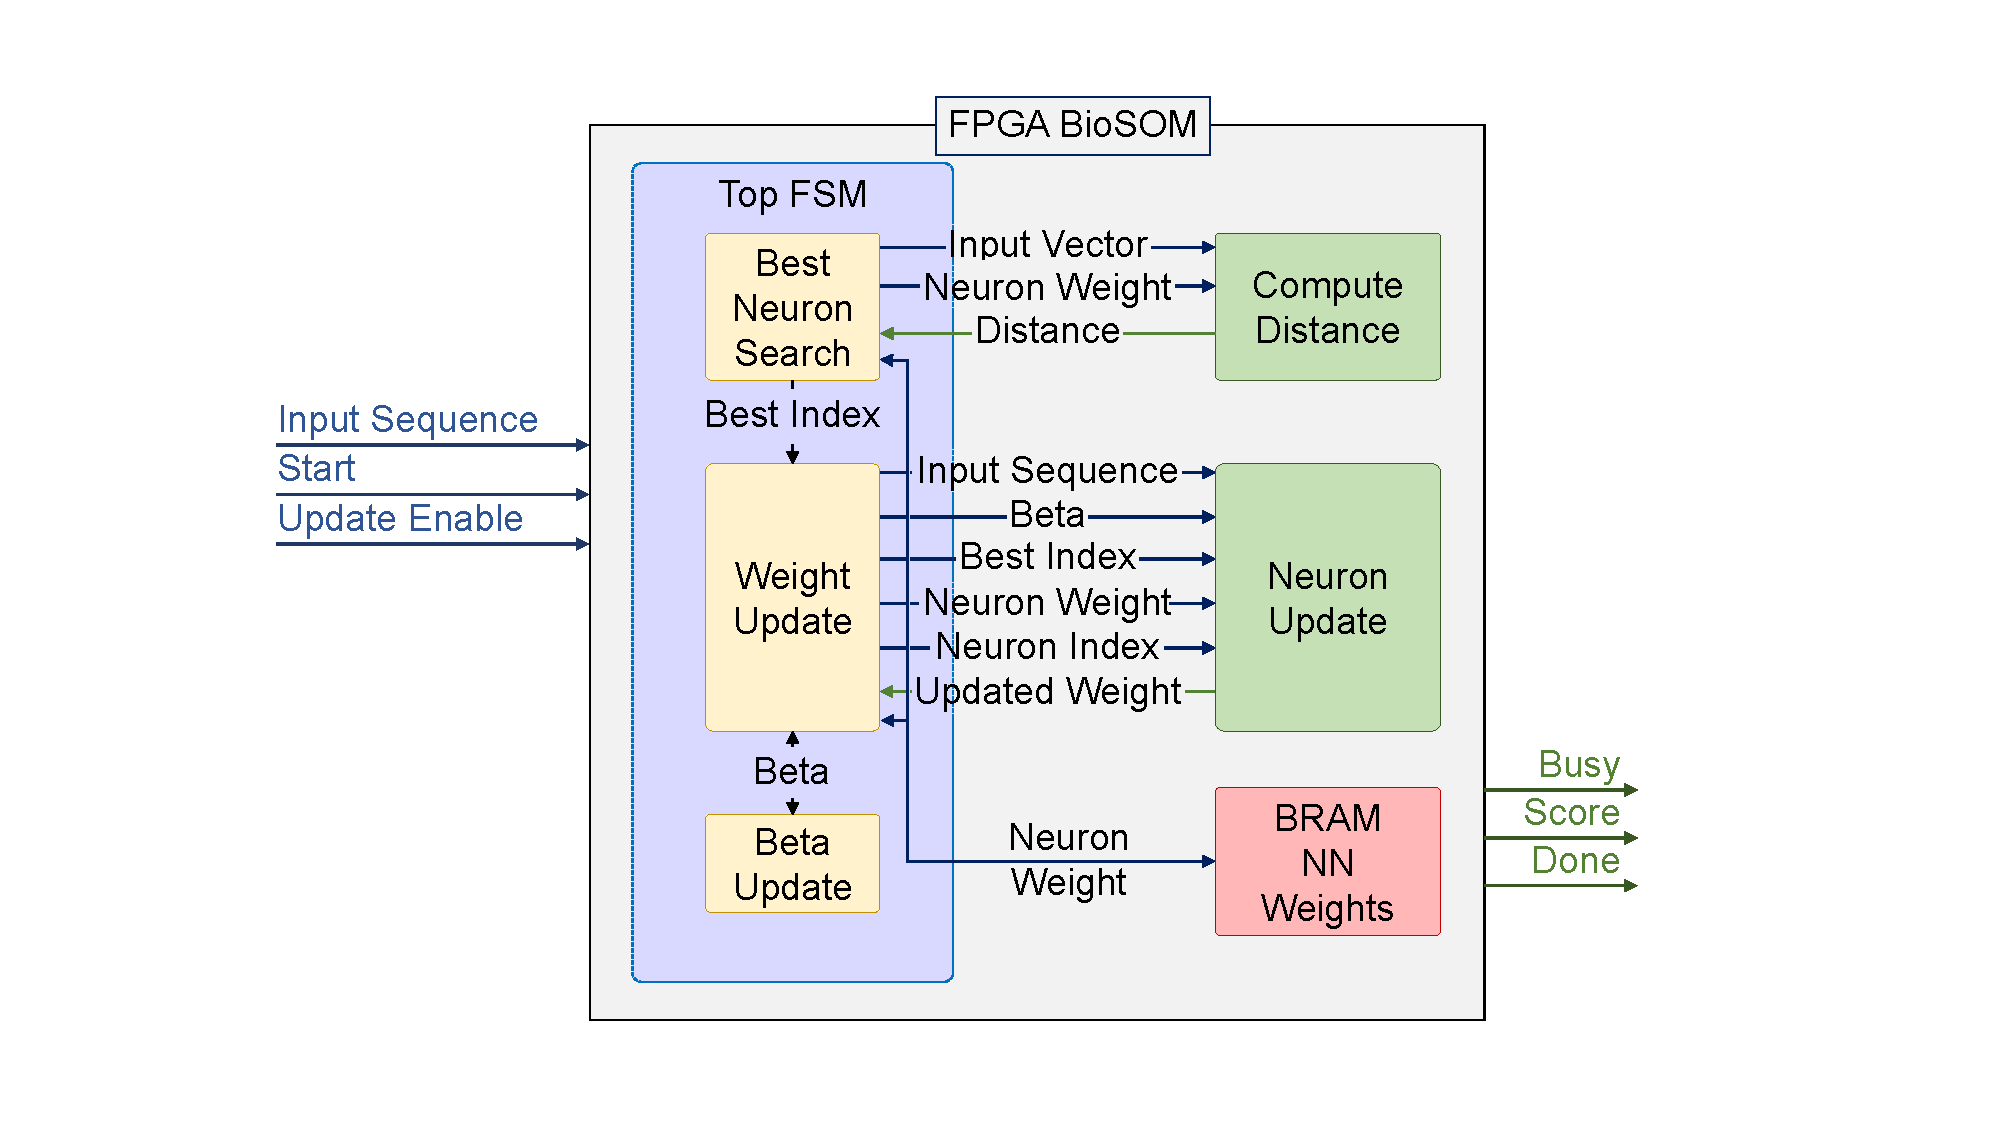
\includegraphics[width=0.49\textwidth]{./somResults/SOMDesignOne_v2}
		\label{fig:algo}}
	\hfil
	\subfloat[]
	{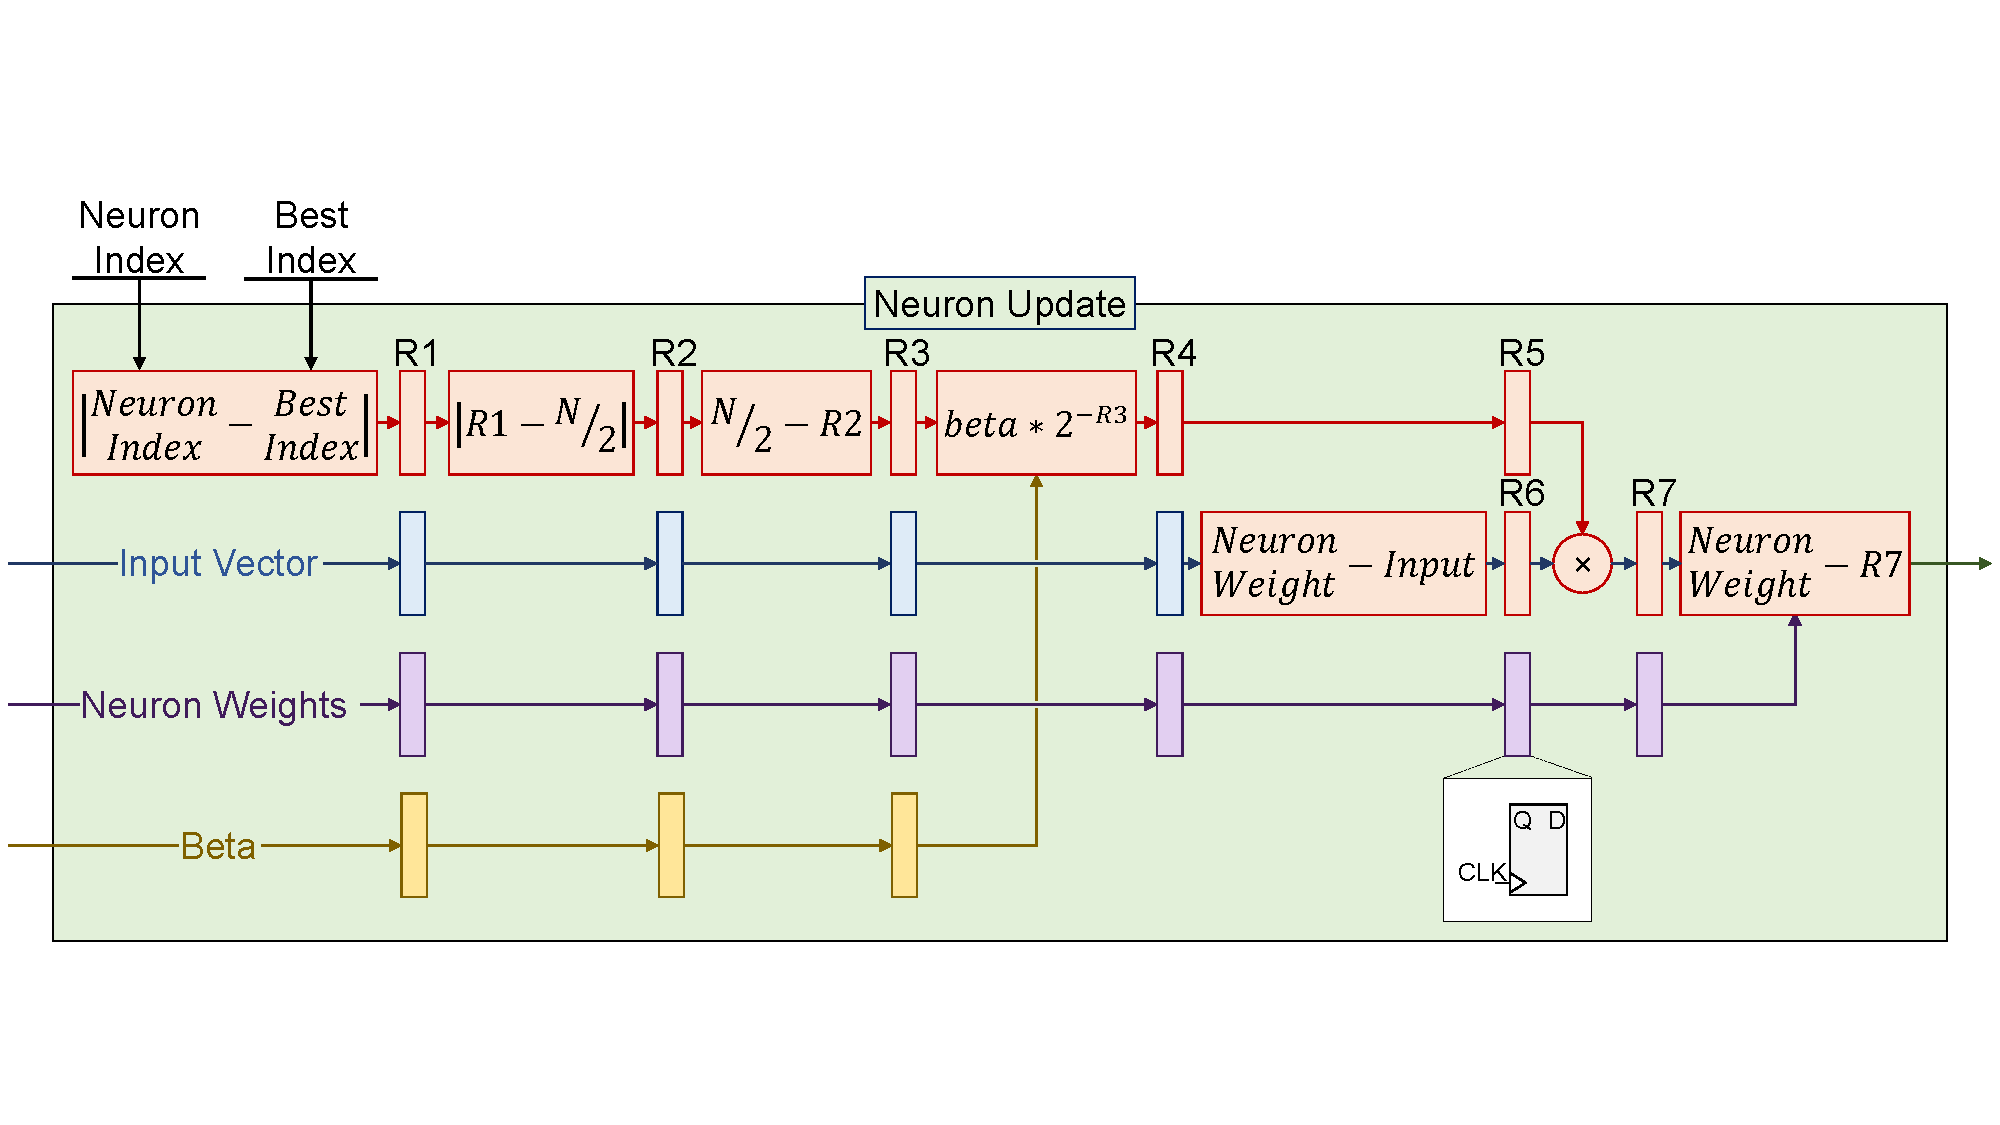
\includegraphics[width=0.49\textwidth]{./somResults/neuronUpdate_v2}
		\label{fig:NeuronUpdate}}
	\caption{(a) Hardware Module for BioSOM. (b) Neuron Update Module.}	\label{fig:SOMFPGAImplementation}
	\vspace{-1.0em}	
\end{figure}

During the training phase \textit{Neuron Update} component is enabled by setting (\textit{Update Enable=1}). The weights of the Neurons are updated using the distance output of the \textit{Compute Distance} module. The \textit{Neuron Update} component is also pipelined design with II=1. The pipeline stages are shown in Figure \ref{fig:NeuronUpdate}.
\subsection{Results}
The SOM has been implemented with a range of fixed-point formats. With fewer bits, one naturally expect that the SOM network to suffer from accuracy degradation. A MATLAB simulation model was created to analyze the accuracy loss when using fixed-point implementation. We trained 10 SOMs with 10 different bacteria DNA sequences. Each SOM network has 100 neurons inside, and each neuron has 20 weights. We trained the networks by two independent training processes running in parallel. One is implemented using double precision floating point and the other is implemented with fixed-point weights. After training, we used the trained networks to identify the unknow sequence and record their scores.

The FPGA design is implemented with Vivado v.2016.4 used for synthesis and analysis of the HDL Designs. Our design is implemented in VHDL and validated using the Vivado simulator. Experimentation is done for different fixed point representations of weights by modifying parameters in VHDL code. 

The area and power numbers for different weight resolutions are extracted from the reports generated by Vivado tool post placement and routing with a working frequency of 100 MHz. Table \ref{table:1} compares the resources and area for 8, 12, 16, 24, and 32 bits fixed point formats, for a SOM network with 512 neurons. The second part of the table compares the average power in the different fixed point formats, for the same SOM.
\begin{table}[!htb]
	\centering
	\caption{Resource Comparison of different fixed point formats}
	\label{table:1}
	\begin{tabular}{ c |c | c| c |c | c } 
		\toprule
		Resource & 8b & 12b & 16b & 24b & 32b \\ 
		\midrule
		LUTs & 1823 & 2611 &3196 & 4375 & 5549 \\
		\hline
		Registers & 3481 & 4679 & 5871 & 8255 & 10639 \\ 
		\hline
		Slice & 854 & 1158 & 1369 &1809 & 2395 \\ 
		\hline
		LUT FF Pairs & 1007 & 1369 & 1750 & 2372 & 3043 \\
		\hline
		B-RAM & 4 & 6 & 8 & 11 & 15 \\
		\hline
		DSP48E1 & 17 & 17 & 17 & 17 & 33 \\
		\hline
		Bonded IOB & 57 & 61 & 65 & 73 & 81 \\
		\midrule
		%    \end{tabular}
	%\end{table}
	
	%\begin{table}[h!]
	%    \centering
	%    \caption{Power Comparison of different fixed-point formats}
	%    \label{table:2}
	%    \begin{tabular}[t]{ c |c | c| c |c | c } 
		\midrule
		Power(W) & 8b & 12b & 16b & 24b & 32b \\ 
		\midrule
		Total Power & 0.295 &0.314 &0.332 &0.356 &0.392 \\
		\hline
		Dynamic &0.052 &0.071 &0.089 &0.113 &0.148 \\ 
		\hline
		Device Static &0.243 &0.243 &0.243 &0.244 &0.244 \\ 
		\bottomrule
	\end{tabular}
\end{table}
\begin{figure}[!htb]
	\centering
	\subfloat[]{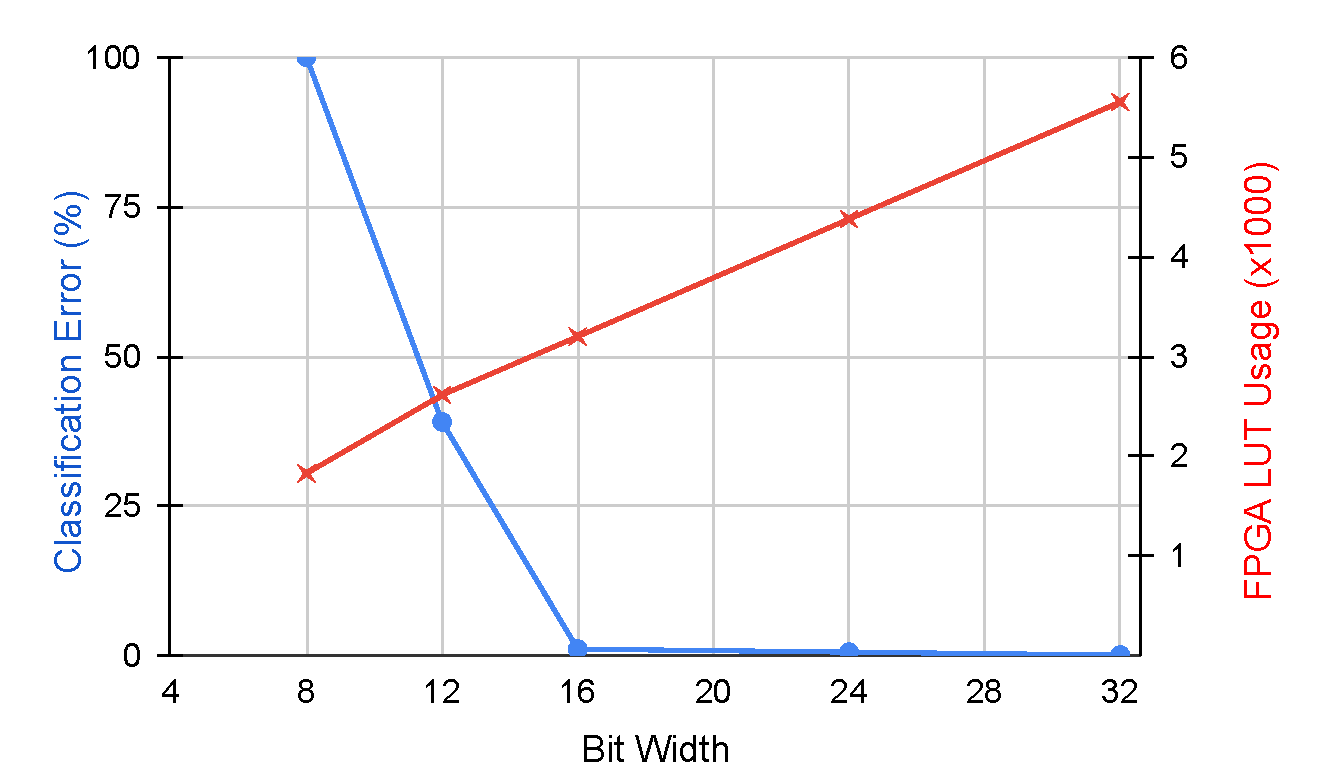
\includegraphics[width=0.45\textwidth]{./somResults/area}
		\label{fig:area}}
	\hfil
	\subfloat[]{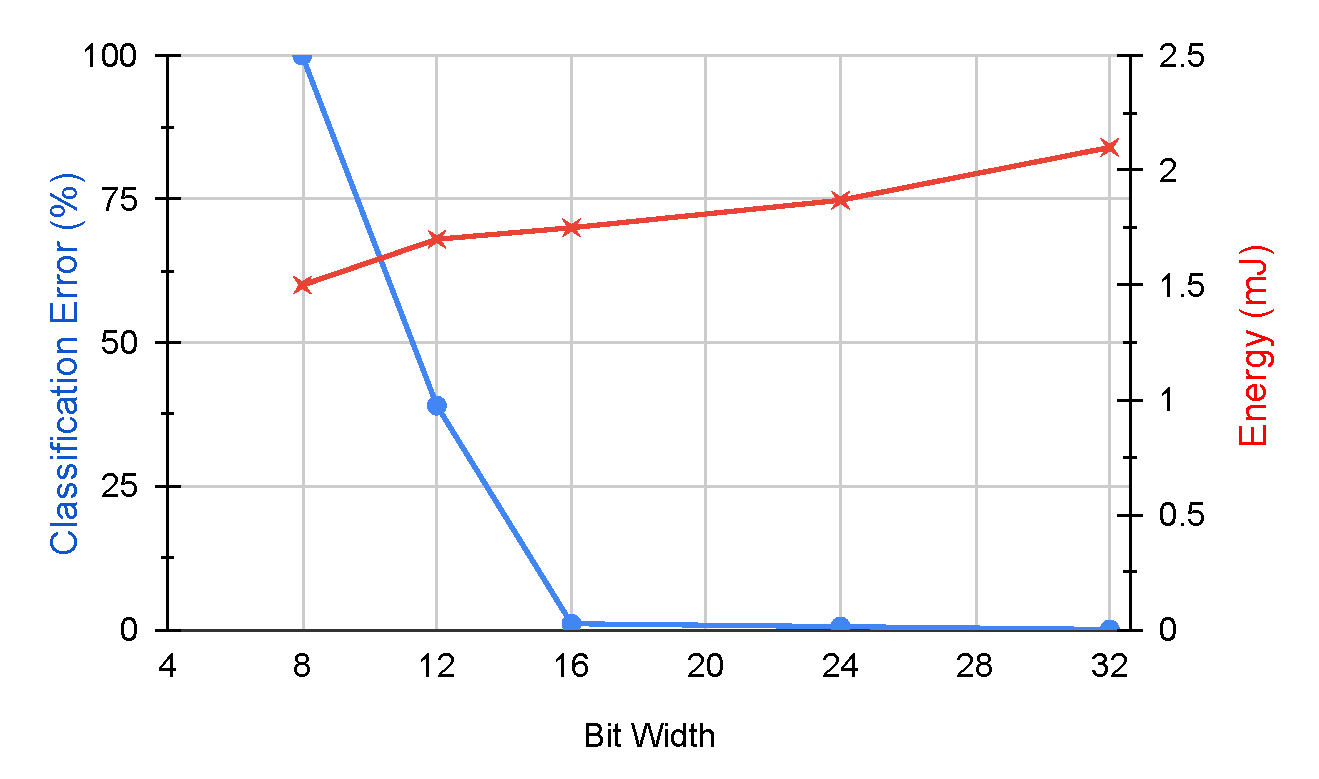
\includegraphics[width=0.45\textwidth]{./somResults/energy}
		\label{fig:energy}}
	\caption{comparison between different fixed-point fromat (a) FPGA LUT utilization (b) energy.}
	\label{fig:metrics}
\end{figure}

The results are summarized in the Figure \ref{fig:area} and \ref{fig:energy}. Both the amount of utilized LUTs and total energy in Joule is presented against the classification error. From the figures, we can easily conclude that, we can substantially reduce the resources used and the energy by using a 16-bit fixed-point representation, without losing accuracy. We can reduce the resources even further by moving to the 12-bit representation, by sacrificing 39\% of the SOM accuracy. 

\section{Conclusion}
With the sudden surge in Neural Network based applications, there is a pressing need for improving the performance and energy efficiency of DNN accelerators for their ubiquitous usage in energy constrained devices. The performance of DNN accelerator's is limited by the memory bandwidth and off-chip memory accesses dominates the energy consumption. The key to improving the energy efficiency of these NNs is reducing the expensive off-chip memory accesses. Towards this we proposed approaches to reduce the off-chip memory accesses for DNNs. The proposed approaches improves the data reuse from on-chip memories for CNNs and LSTMs by partioning the data and scheduling the operations. We have also analyzed the impact of low bit resolution on the accuracy and energy, area performance for NNs. 

\footnotesize
\bibliographystyle{abbrv} %IEEEtran % abbrv
%\vspace{1.5mm}
\bibliography{refs}
%\nocite{*}
%\end{spacing}

\end{document}
